\chapter{Designing and Implementing the OurPlace platform}
\label{chap:Design}

\section{Overview}
In this paper, we contribute insights gained from longitudinal studies of place-based m-learning in two contexts: formal education and informal, community-led learning. Additionally, we present ParkLearn: a m-learning platform designed to support teachers, students and communities in creating, sharing and engaging with bespoke m-learning activities. We report on how ParkLearn was used by teachers and community experts in these two learning contexts, supporting both groups in achieving their own disparate goals through the democratisation of m-learning activity design. We discuss how m-learning technologies can support empowerment through encouraging creativity and content ownership; promote civic engagement and inquiry; and assist in seamless learning teaching practices by being an adaptable, supporting toolkit.

We build upon the aforementioned engagements held by Richardson et al. [29] by using the design contexts of primary schools and nearby local parks as applicable examples of formal and informal learning environments. A primary school setting was chosen due to the national curriculum being less restrictive during the earlier school years, allowing teachers to experiment more with lesson planning and perform more outdoor activities. Parks were chosen as they have traditionally been used as outdoor learning resources by nearby schools. However, prolonged austerity measures have meant that local councils have resorted to cutting dedicated educational staff in their parks or introducing fees for the use of park rangers’ time. As a result, the UK’s parks are becoming an increasingly underutilised learning resource.

\section{Technology Design Goals}

Based on the findings of previous works [16,33,39,40,42] and the design engagements held by Richardson et al. [29], we produced several design goals (DGs):
DG1.	Utilize local places and communities as learning resources—give places’ stakeholders a platform for sharing their values through designing and sharing learning activities in authentic contexts [22,29].
DG2.	Support seamless outdoor and classroom use by encompassing as many of Wong and Looi’s [43] desirable dimensions of seamless learning as possible (such as using multiple device types across locations).
DG3.	Be flexible enough to support different goals, learning processes and intended outcomes without relying on additional tools (e.g. provide evidence of learning output for teachers or promote placemaking [29]).
DG4.	Support a wide range of user ages and technical expertise through simple, consistent visual interfaces [21] which reduce the need for typing [40].
DG5.	Utilise interaction methods which support creativity, control [14] and allow for immediate activity creation, data collection and reflection in authentic learning contexts (in contrast to MyArtSpace [40]).
DG6.	Support mobile learning in resource-limited schools through allowing device sharing (as seen in Mobilogue [16]) and offline caching of data.
With these design goals in mind, we created ParkLearn: a platform designed to lower the barrier to entry of creating rich mobile learning content.  The following sections of this paper will give a brief overview of the ParkLearn platform, before describing how it was used in two user studies to evaluate it against these design goals.

\section{The Anatomy of an Activity}
\label{sec:ActivityOverview}

\section{Development of the Technology}

\subsection{Why use the Xamarin framework?}
The OurPlace platform is a system consisting of smartphone applications for the
Android and iOS (Apple iPhone and iPad) operating systems, a website and an
online application programming interface (API). It was decided that in order to
support as many schools, groups and individuals as possible, both of the main
smartphone OSs should be supported (Android and iOS). Furthermore, in order to
provide a high quality experience which conformed to each platform's expected
design metaphors,  supported access to all of the devices' hardware features and
didn't require a constant internet connection, I decided to produce `native'
applications for each platform (that is, rather than produce something like a
website which would be the same across all platforms). Ordinarily, this would
result in having to produce software in multiple programming languages: for
example, Android applications are usually written in either Java or Kotlin,
whereas iPhone apps are written in Objective-C, which is very different. As the
project was mostly a one-man show, dedicating large amounts of time to learning,
developing, iterating and maintaining systems across multiple languages was
unrealistic. 

In the end, the decision was made to develop the mobile applications using the
Xamarin framework. This framework takes code written in C\# and compiles it into
`native' applications, meaning that apps look, feel and act like software
written in the different platforms' specific languages. This gave the advantage
of sharing the same programming language across both applications, without
losing out on any major features and allowing for common code (functionality
identical across the two applications, e.g. making requests to the server) to be
shared across the projects. To fully capitalise on this code sharing advantage,
it was decided to take this further and produce the website and API in C\#. As a
result, every component of the OurPlace platform can be opened within the same
Visual Studio `solution', significantly speeding up the development process.

\subsection{Disadvantages to using Xamarin}
While developing the mobile applications with the Xamarin framework
significantly reduced to upfront time investment in the development process, it
certainly had its trade-offs which became more apparent as the project grew.
Having all of the OurPlace code available within one solution (discussed in
\ref{sec:OurPlaceSolution}) was certainly convenient and minimised code
duplication, but when combined with Xamarin's more demanding build process it
created large performance overheads. This, combined with issues of documentation
being in other programming languages (particularly on the iOS application),
impeded the development workflow, frequently slowing it to a crawl. At the end
of the project, it is difficult to say if significant time was saved by using
Xamarin over the two platforms' `native' development tools. However, anyone
considering these options should note that recent developments to Visual Studio
and the Xamarin framework have significantly improved performance, which may somewhat
mitigate these issues.

\subsection{A Brief Tour of the OurPlace Visual Studio Solution}
\label{sec:OurPlaceSolution}
All of the OurPlace code is open source, and can be viewed at
\url{https://github.com/GSDan/OurPlace}. Using C\# and Microsoft's .NET Framework
across the OurPlace platform afforded it being accessible within a single Visual
Studio solution, split into four smaller component projects:
\textit{OurPlace.Common}, \textit{OurPlace.API}, \textit{OurPlace.Android} and
\textit{OurPlace.iOS}.

\paragraph{OurPlace.Common}
This is a .NET Standard 2.0 project, which acts as a `library' of functions and
serves the other projects within the solution. It contains shared data models,
interfaces and common core functionality, including managing the apps' local
files, authenticating with the server, polling it for the latest OurPlace
activities and uploading new activities and responses. This is the only project
which is referenced from elsewhere in the solution.

\paragraph{OurPlace.API}
This project uses version 4.6.1 of the .NET Framework, and contains an ASP .NET
website, a Web API 2 powered API and a Code First, Entity Framework database.
This project is discussed in detail in section \ref{sec:ImplementationWeb}.

\paragraph{OurPlace.Android}
This project contains all of the code specific to the Android application.
Written in C\# using the Xamarin.Android framework, a `native' Android application is
produced upon compilation, supporting devices running Android versions as old as
4.1 (Jelly Bean, 2012) and targeting the latest features found in version 8.1
(Oreo, 2017). This project is discussed in detail in section
\ref{sec:ImplementationMobile}.

\paragraph{OurPlace.iOS}
This project contains all of the code specific to the iPhone/iPad application.
Written in C\# using the Xamarin.iOS framework, a `native' iOS application is
produced upon compilation. The application requires a minimum of iOS 10, which
is supported by devices as old as the iPhone 5 (released 2012). This project is
discussed in detail in section \ref{sec:ImplementationMobile}.

\section{Implementation of the API and Website}
\label{sec:ImplementationWeb}

\section{Implementation of the ParkLearn Application}
\label{sec:ImplementationParkLearn}

The first version of OurPlace, called ParkLearn, was produced as a prototype
Android app. This early version was created as a proof of concept, digitising
the format of the jigsaw workshop activity (discussed in section
\todo[inline]{reference discussion of jigsaw workshop activity}). The prototype
supported the completion of pre-created interactive activities, following the
format discussed in \ref{sec:ActivityOverview}. However, follow-up tasks had not
yet been implemented, nor had the `\textit{Scan the QR Code}', `\textit{Listen to
Audio}' and `\textit{Information}' task types.

\subsection{Creating Activities}

\subsection{Sharing, Discovering and Launching Activities}

\subsubsection{The Highlights Feed and Location}

\subsubsection{Share Codes and QR Codes}

\subsection{Completing Activities}

\section{Implementation of the OurPlace Mobile Applications}
\label{sec:ImplementationMobile}

\subsection{Improvements over ParkLearn}

\subsubsection{Developing the iOS Application}

\subsubsection{Adding Follow-Up Tasks}

\subsubsection{QR Code Task Types}

\subsubsection{Other General Improvements}


\subsection{The OurPlace App}

OurPlace is the current iteration of the open-source ParkLearn platform, with an expanded feature set and re-branded to support its use in contexts outside of local parks \citep{Richardson2018a}. Consisting of a website and mobile applications for both Android and iOS, OurPlace supports the creation of--and sharing and engagement with--m-learning activities (`Activities'), each of which is built up from smaller, modular tasks (`Tasks'). These tasks each consist of a specific interaction (`Task Type'), which either promote creativity, emulate traditional classroom learning materials or use the device's hardware to give context-specific experiences (Table~\ref{tab:TaskTypes}). With the exception of \textit{Scan the QR Code}, all of these Task Types were present in the original ParkLearn application. OurPlace also adds support for `Follow-Up Tasks', which allow activity creators to add sub-tasks which unlock once their parent task has been completed (Figure~\ref{fig:ActivityCreation}.e). This supports the design of more complicated combinations of interactions (for example: a \textit{Location Hunt} could unlock a \textit{Record Audio} and \textit{Take a Photo} once the user arrives at a designated location).

\begin{table}
  \centering
  \begin{tabular}{l|p{110mm}}
    % \toprule
    {\small\textit{Task Type}}
    & {\small \textit{Interaction Description}} \\
    \midrule
    \small Information & \small Read some written information, with an optional accompanying image and hyperlink \\
    \small Listen to Audio & \small Listen to a given audio recording \\
    \small Take a Photo & \small Use the camera to take still images \\
    \small Photo Match & \small Use the camera to match an existing photo given as an overlay \\
    \small Draw a Picture & \small Draw a picture onto a blank canvas \\
    \small Draw on Photo & \small Draw on top of a given image \\
    \small Record Video & \small Record a video using the camera \\
    \small Record Audio & \small Record audio using the device's microphone \\
    \small Map Marking & \small Mark a given number of locations onto a Google Map \\
    \small Location Hunt & \small Track down a target location by observing your reported distance \\
    \small Scan the QR Code & \small Find and scan the correct QR code \\
    \small Multiple Choice & \small Choose a response from text options \\
    \small Text Entry & \small Enter a response using the keyboard
    % \bottomrule
  \end{tabular}
  \caption{The Task Types available in the OurPlace application}~\label{tab:TaskTypes}
\end{table}

\begin{figure*}
  \centering
  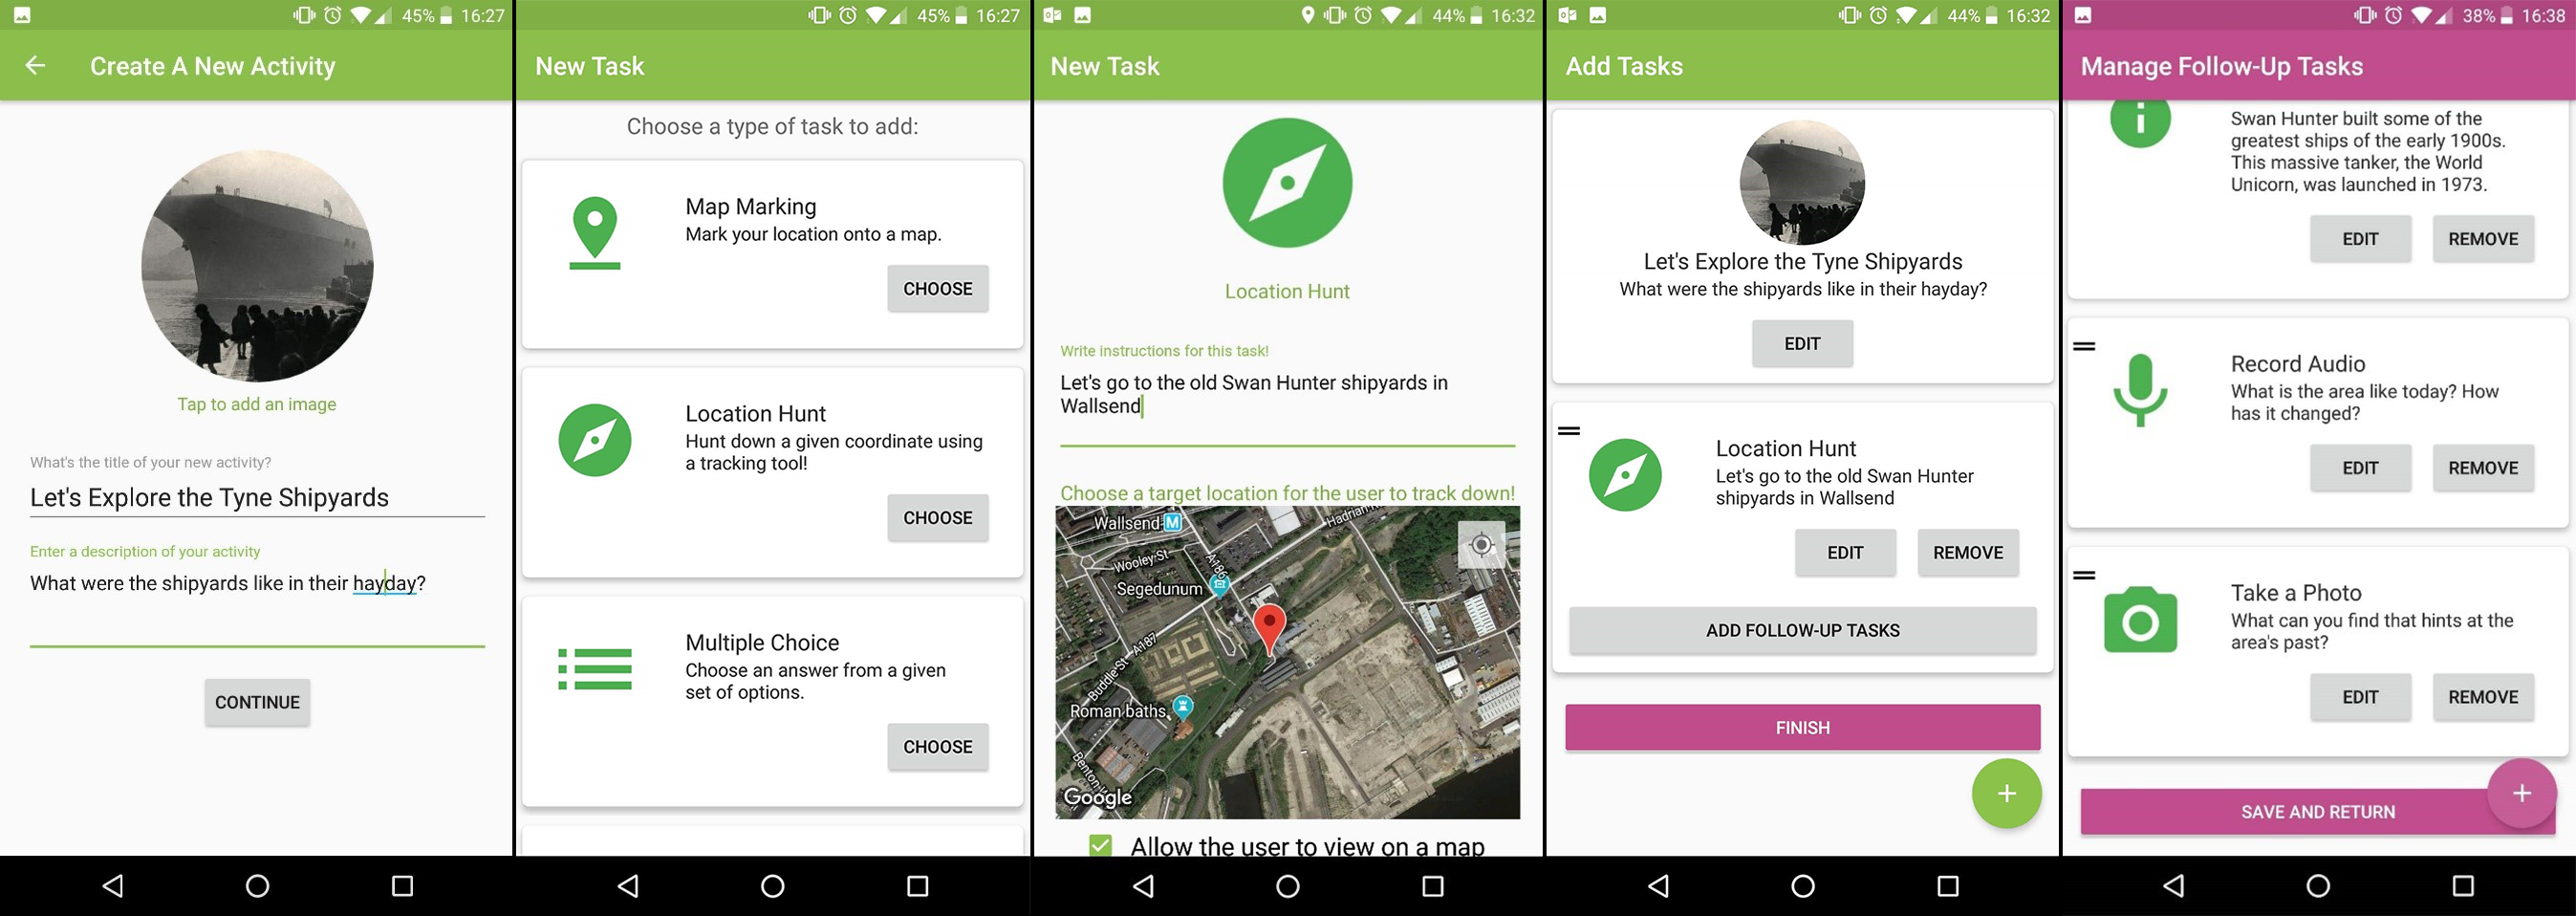
\includegraphics[width=1\columnwidth]{images/chapter08/activityCreation}
  \caption{Creating an OurPlace activity (left to right): a) Choosing the activity's title, description and image; b) Choosing a Task Type to add; c) Adding a \textit{Location Hunt} Task, with description and target coordinates; d) The new Task in the Activity; e) Adding Follow-Up Tasks to the \textit{Location Hunt}  }~\label{fig:ActivityCreation}
\end{figure*}

Activities are created within the app itself. After supplying a title, description and an optional image (Figure~\ref{fig:ActivityCreation}.a), the designer creates the Tasks that make up the Activity (Figure~\ref{fig:ActivityCreation}.b). Each Task Type requires at least a written instruction for the learner (e.g. A \textit{Location Hunt} might say \textit{`Can you find Carter's Well?'}), but some of them require some additional customization (e.g. supplying geographic coordinates by tapping on a Google Maps view) (Figure~\ref{fig:ActivityCreation}.c). No additional equipment or software is required to create activities (other than \textit{Scan the QR Code}, which requires creators to print the generated QR code from the OurPlace website). Uploaded activities can be edited for testing, feedback and iteration--allowing for the `essential elements' of reflection, critique and revision of a final public product \citep{Larmer2015}. 